\documentclass[a4paper,12pt]{article}
\AtBeginDocument{\fontsize{14pt}{21pt}\selectfont}
\usepackage{fontspec}
\setmainfont{Times New Roman}
\newfontfamily\cyrillicfont{Times New Roman}
\newfontfamily\englishfont{Times New Roman}
\newfontfamily\cyrillicfonttt{Times New Roman}
\usepackage{polyglossia}\setdefaultlanguage{russian}\setotherlanguage{english}
\usepackage[left=30mm,right=15mm,top=20mm,bottom=20mm]{geometry}
\usepackage{setspace}\onehalfspacing
\usepackage{indentfirst}\setlength{\parindent}{1.25cm}\setlength{\parskip}{0pt}
\usepackage{graphicx,amsmath,amssymb,booktabs,array,longtable,caption}
\usepackage[hidelinks]{hyperref}
\usepackage[backend=biber,style=gost-numeric,sorting=none,language=auto]{biblatex}\addbibresource{refs.bib}
\usepackage{titlesec}\titleformat{\section}{\centering\normalfont\bfseries\Large}{\thesection.}{0.5em}{}\titlespacing*{\section}{0pt}{0pt}{12pt}\titleformat{\subsection}{\normalfont\bfseries\large}{\thesubsection.}{0.5em}{}\titlespacing*{\subsection}{0pt}{12pt}{6pt}
\captionsetup{font=normalsize,labelfont=normalfont,justification=centering}
\begin{document}
\begin{titlepage}\thispagestyle{empty}\begin{center}\bfseries Московский авиационный институт\\Институт компьютерных наук (Институт №8)\vfill\Large ОТЧЕТ ПО КУРСОВОМУ ПРОЕКТУ\par\vspace{8mm}\normalsize\textbf{«Нечеткие величины на основе равномерного закона U(a,b): генерация, операции над α-срезами и кластеризация»}\vfill\begin{flushleft}\normalfont Дисциплина: «Неклассические логики»\\Руководитель: Д. В. Кубраков, преподаватель ОЦ-8\\Студент: \rule{6cm}{0.4pt}\quad Группа: \rule{2.5cm}{0.4pt}\end{flushleft}\vfill Москва, 2026\end{center}\end{titlepage}
\setcounter{page}{2}\tableofcontents\clearpage
\section*{Введение}\addcontentsline{toc}{section}{Введение}Курсовой проект посвящён разработке программного комплекса для представления и анализа нечётких величин, заданных на основе равномерного закона \(U(a,b)\). Исходная постановка требует независимой библиотеки, способной генерировать наборы величин, выполнять арифметические операции, отбирать элементы по критериям и проводить кластерный анализ. В проекте эта задача решена разделением математического ядра на C++ и клиентского слоя на Go, связанного с ядром через C API и cgo.

Актуальность работы определяется тем, что интервальные и нечёткие данные возникают при измерениях, экспертном оценивании и моделировании систем с неполной информацией. Скалярная обработка скрывает ширину неопределённости, тогда как \(\alpha\)-срез сохраняет её в форме вложенного интервала. Такое представление позволяет единообразно выполнять арифметику и переносить задачу кластеризации в пространство пар границ \((A,B)\). Для достоверной проверки алгоритмов требуется воспроизводимый генератор, поэтому в ядре реализован собственный генератор xoshiro256** с инициализацией splitmix64.

Цель работы состоит в создании и исследовании программного комплекса, который формирует нечёткие величины вида \(U(a,b)\), вычисляет их \(\alpha\)-срезы и кластеризует полученные интервалы. Для достижения цели необходимо формализовать модель принадлежности, реализовать интервальную арифметику и операции сравнения, обеспечить генерацию наборов размером от 100 до 300 элементов, реализовать два алгоритма кластеризации и предоставить внешний интерфейс для браузерного и десктопного клиентов.

Объектом исследования является программная система обработки нечётких величин и множеств таких величин. Предмет исследования составляют структуры данных и алгоритмы, реализованные в каталогах \texttt{fuzzy/}, \texttt{server/} и \texttt{desktop/}. При подготовке отчёта использованы исходные файлы проекта, документация \texttt{docs/theory.md}, \texttt{docs/library\_api.md}, тест \texttt{fuzzy/tests/test\_main.cpp} и задание на практику.

В работе используется важное соглашение модели. Равномерный закон \(U(a,b)\) задаёт вероятностный диапазон и плотность \(f(x)=1/(b-a)\) на \([a,b]\). Функция принадлежности в проекте выбрана отдельно: это нормированная функция распределения, линейно возрастающая от 0 до 1 на том же носителе. Поэтому термин «на основе равномерного закона» относится к исходным параметрам и носителю, а \(\mu(x)\) является функцией нечёткой модели, а не плотностью вероятности.

Отчёт состоит из четырёх глав. В первой формулируются проблема, цель, задачи и границы применимости. Во второй вводятся математический аппарат \(\alpha\)-срезов, интервальная арифметика, генератор и алгоритмы кластеризации. Третья глава описывает архитектуру C++-ядра, C API, Go-сервера и пользовательских оболочек. В четвёртой приводятся методика тестирования, контрольные измерения, результаты кластеризации и ограничения экспериментальной проверки.
\clearpage
\section{Глава 1. Введение и постановка задачи}\subsection{Актуальность темы}

Во многих задачах анализа данных исходные сведения задаются не точками, а диапазонами. Левая и правая границы интервала могут отражать разброс измерения, неопределённость эксперта или неполноту наблюдения. При этом одинаковое отношение ко всем значениям внутри диапазона часто оказывается слишком грубым. Нечёткая величина позволяет присвоить каждому значению степень принадлежности от 0 до 1 и тем самым сохранить информацию о постепенном переходе от маловероятных к предпочтительным значениям.

Практическая ценность такого представления проявляется в задачах, где требуется сопоставлять неопределённые объекты, выполнять арифметические преобразования и выделять компактные группы. В рассматриваемом проекте нечёткая величина строится из параметров равномерного закона U(a,b). На выбранном уровне α она преобразуется в интервал [A,B], после чего интервалы можно сравнивать, отбирать и кластеризовать. Такое преобразование связывает аппарат нечётких множеств с классическими алгоритмами обработки данных на евклидовой плоскости границ.

Проблема кластеризации в данном случае состоит в том, что объектом анализа является не скаляр, а отрезок. Расстояние должно учитывать обе границы, а центр кластера должен иметь интерпретируемый вид. В библиотеке используется метрика Хаусдорфа для интервалов, которая сводится к максимуму модулей разностей левой и правой границ. Это сохраняет геометрический смысл расстояния и позволяет применять адаптированные варианты k-means++ и пороговой кластеризации.

Отдельную вычислительную проблему создаёт необходимость воспроизводимой генерации наборов. Библиотека не использует внешние генераторы случайных величин. В \texttt{fuzzy/src/rng.cpp} реализованы xoshiro256** и инициализация состояния через splitmix64. Один и тот же seed формирует один и тот же поток псевдослучайных чисел, что необходимо для воспроизводимого эксперимента и сравнения алгоритмов.

\subsection{Объект, предмет и исходные данные проекта}

Объектом исследования является программная система для работы с наборами нечётких величин вида U(a,b) и их α-срезами. Предмет исследования составляют алгоритмы представления, генерации, арифметического преобразования, отбора и кластеризации интервалов.

Исходный код проекта разделён на следующие части:

\begin{itemize}
\item математическое ядро в каталоге \texttt{fuzzy/}, включающее C++17-реализацию типов \texttt{fz\_number}, \texttt{fz\_set}, \texttt{fz\_rng}, арифметики, отбора и кластеризации;
\end{itemize}

\begin{itemize}
\item C API в файле \texttt{fuzzy/include/fuzzy.h}, через который ядро вызывается из внешних языков;
\end{itemize}

\begin{itemize}
\item Go-сервер в каталоге \texttt{server/}, хранящий состояние набора, проверяющий HTTP-запросы и преобразующий данные между JSON, Go-структурами и C API;
\end{itemize}

\begin{itemize}
\item веб-интерфейс \texttt{server/web/}, встроенный в исполняемый файл Go посредством \texttt{go:embed};
\end{itemize}

\begin{itemize}
\item десктопная оболочка \texttt{desktop/}, запускающая локальный сервер и отображающая тот же интерфейс через CEF.
\end{itemize}

Документация \texttt{docs/theory.md} и \texttt{docs/library\_api.md} фиксирует математические определения и контракт внешнего интерфейса. Тестовый набор \texttt{fuzzy/tests/test\_main.cpp} содержит проверки α-срезов, арифметики, генератора, отбора и кластеризации.

\subsection{Цель и задачи курсового проекта}

Цель проекта состоит в разработке и исследовании программного комплекса, который воспроизводимо генерирует нечёткие величины U(a,b), вычисляет их α-срезы и выполняет кластеризацию полученных интервалов с единым C API для C++, Go и других языков.

Для достижения цели решены следующие задачи:

\begin{enumerate}
\item Формализована нечёткая величина в виде функции принадлежности и набора вложенных α-срезов.
\item Реализованы параметрическое представление U(a,b) и дискретное представление произвольной величины через массивы левых и правых границ.
\item Реализованы сложение, вычитание, умножение и деление по интервальной арифметике на каждом уровне α.
\item Реализованы центр тяжести и сравнение по степени возможности.
\item Реализованы xoshiro256**, splitmix64 и генерация наборов с контролируемыми диапазонами начальной точки и ширины.
\item Реализованы отбор по ширине α-среза и по заданному окну.
\item Реализованы k-means++ с заданным числом кластеров и пороговая кластеризация с автоматически определяемым числом кластеров.
\item Создан Go-слой с cgo, HTTP API, импортом и экспортом CSV, журналом и синхронизацией состояния.
\item Проведены модульная верификация и контрольные измерения времени исполнения.
\end{enumerate}

\subsection{Границы применимости}

Библиотека принимает конечные вещественные параметры и проверяет условие \texttt{a < b}. Число уровней задаётся в диапазоне от 2 до 10001, а число генерируемых элементов ограничено диапазоном от 1 до 100000. В Go-сервере выбран фиксированный размер сетки из 21 уровня. Этот режим соответствует интерфейсному сценарию и уменьшает объём передаваемых данных.

Рассматриваемая форма функции принадлежности является монотонно возрастающим треугольником на [a,b]. Для результатов арифметических операций библиотека хранит общую нечёткую величину как вложенные интервалы. Деление запрещается, если носитель делителя содержит ноль. Кластеризация работает с α-срезами одного выбранного уровня, поэтому она не заменяет многомасштабный анализ по нескольким α, а предоставляет анализ фиксированного уровня неопределённости.

Алгоритмы рассчитаны на работу в памяти процесса. Сервер хранит одно текущее состояние набора, защищённое \texttt{sync.Mutex}. Персистентное хранилище, распределённая обработка и межпроцессная база данных в проект не входят.

\begin{figure}[htbp]\centering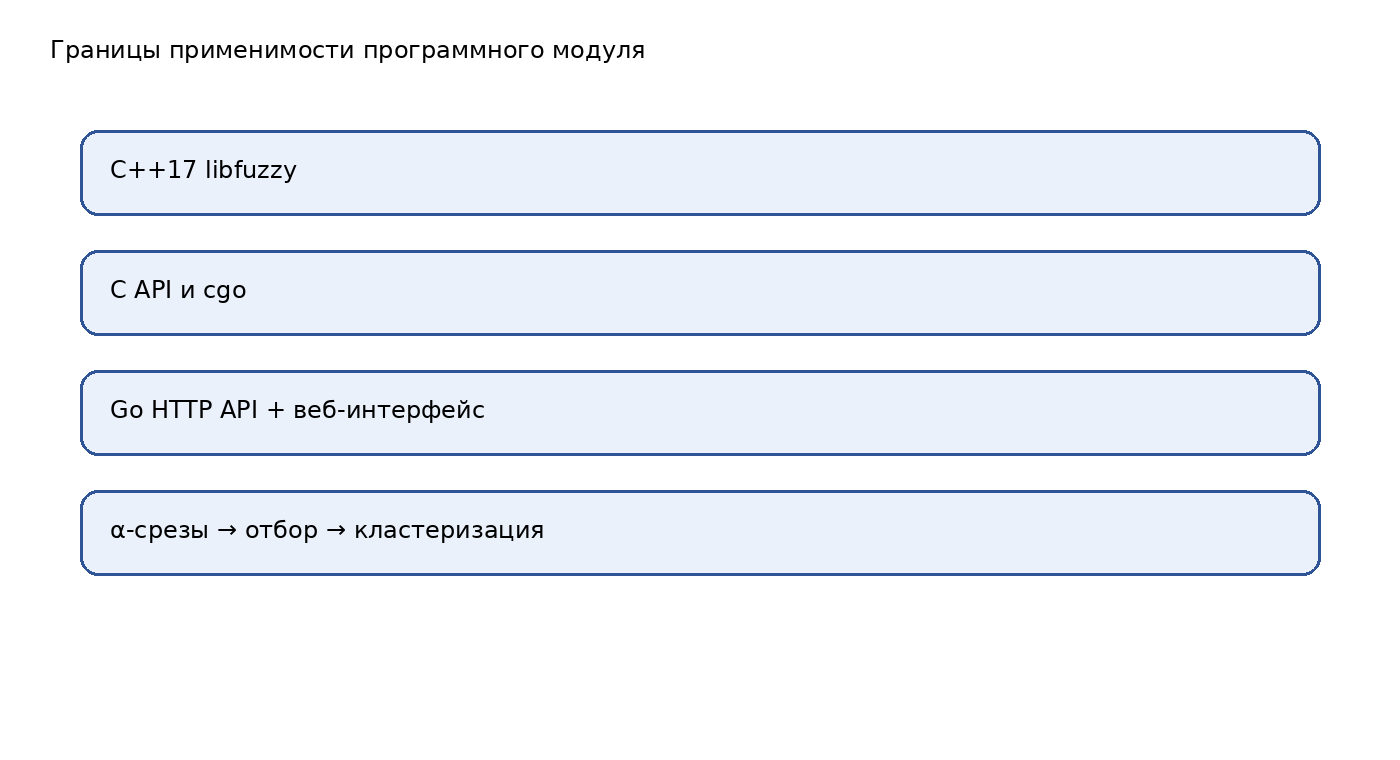
\includegraphics[width=0.9\textwidth]{figures/fig1_scope.png}\caption{схема границ применимости программного модуля}\label{fig:1}\end{figure}

---\clearpage
\section{Глава 2. Теоретические и алгоритмические основы}\subsection{Формализация нечёткой величины}

Нечёткая величина X на множестве действительных чисел задаётся функцией принадлежности

\begin{equation}
\mu_X: \mathbb{R}\rightarrow[0,1],
\end{equation}

где значение μ\_X(x) выражает степень принадлежности числа x величине X. Носитель и ядро определяются как

\begin{equation}
\operatorname{supp}X=\{x\mid \mu_X(x)>0\},\qquad \operatorname{core}X=\{x\mid \mu_X(x)=1\}.
\end{equation}

Для $\alpha\in[0,1]$ $\alpha$-срез имеет вид

\begin{equation}
X_\alpha=\{x\in\mathbb{R}\mid \mu_X(x)\geq\alpha\}.
\end{equation}

Для нормальной выпуклой величины каждый срез является отрезком [L(α),R(α)]. Вложенность срезов выражается условием

\begin{equation}
\alpha_1<\alpha_2 \Rightarrow X_{\alpha_2}\subseteq X_{\alpha_1},
\end{equation}

что в дискретном представлении проверяется неубыванием левых границ и неувеличением правых границ. Теорема о декомпозиции позволяет восстановить функцию принадлежности по семейству срезов:

\begin{equation}
\mu_X(x)=\sup\{\alpha\mid x\in X_\alpha\}.
\end{equation}

В структуре \texttt{fz\_number} это семейство хранится в векторах \texttt{left} и \texttt{right}. Для исходной величины дополнительно сохраняются \texttt{uniform}, \texttt{a} и \texttt{b}, что позволяет использовать точные формулы без обращения к дискретной сетке.

\subsection{Равномерный закон U(a,b) как исходная нечёткая величина}

Для a<b равномерное распределение задаётся плотностью

\begin{equation}
f(x)= \begin{cases} \frac{1}{b-a}, & a\leq x\leq b,\\ 0, & \text{иначе}. \end{cases}
\end{equation}

В проекте в качестве функции принадлежности используется нормированная линейная функция на том же носителе:

\begin{equation}
\mu_{U(a,b)}(x)= \begin{cases} \frac{x-a}{b-a}, & a\leq x\leq b,\\ 0, & \text{иначе}. \end{cases}
\end{equation}

Она возрастает от нуля в точке a до единицы в точке b. Носитель равен [a,b], ядро — одноточечное множество \{b\}. На уровне α левая граница определяется как

\begin{equation}
L(\alpha)=a+\alpha(b-a),
\end{equation}

а правая граница постоянна:

\begin{equation}
R(\alpha)=b.
\end{equation}

Следовательно,

\begin{equation}
U(a,b)_\alpha=[a+\alpha(b-a),b], \quad |U(a,b)_\alpha|=(1-\alpha)(b-a).
\end{equation}

В \texttt{make\_uniform} эта зависимость вычисляется для всех \texttt{levels} значений сетки α\_i=i/(m−1). Для U(a,b) дискретизация не вносит аппроксимационной ошибки в положение левой границы, так как функция L(α) линейна. Для результатов операций срез на промежуточном уровне получают линейной интерполяцией.

Центр тяжести исходной величины вычисляется аналитически:

\begin{equation}
c_X=\frac{\int_a^b x\mu_X(x)\,dx}{\int_a^b\mu_X(x)\,dx} =a+\frac{2}{3}(b-a).
\end{equation}

Для величин общего вида \texttt{fz\_centroid} применяет численное интегрирование по 2000 равным шагам с трапецеидальными весами. Если площадь под функцией принадлежности вырождается, возвращается середина носителя.

\subsection{Концепция α-уровней в кластеризации}

α-срез переводит нечёткое число в интервал, который содержит значения с принадлежностью не ниже выбранного порога. При α=0 анализируется полный носитель. При α=1 для U(a,b) срез вырождается в точку b. Таким образом, увеличение α уменьшает неопределённость и смещает левую границу к правой.

Для каждого элемента набора на фиксированном α формируется пара

\begin{equation}
P_i=(A_i,B_i)=(L_i(\alpha),R_i(\alpha)).
\end{equation}

Кластеризация выполняется на этих парах. Геометрическое расстояние между отрезками определяется формулой

\begin{equation}
d_i= d([A_1,B_1],[A_2,B_2])= \max\left(|A_1-A_2|,|B_1-B_2|\right).
\end{equation}

Эта функция совпадает с расстоянием Хаусдорфа для компактных интервалов на прямой. Представление P\_i на плоскости делает левую границу координатой x, а правую границу координатой y. Центр кластера является парой средних координат

\begin{equation}
C_j=\left(\frac{1}{n_j}\sum_{i\in K_j}A_i, \frac{1}{n_j}\sum_{i\in K_j}B_i\right).
\end{equation}

Разброс кластера вычисляется как среднеквадратичное расстояние:

\begin{equation}
s_j=\sqrt{\frac{1}{n_j}\sum_{i\in K_j}d(P_i,C_j)^2}.
\end{equation}

Поэтому центр и разброс имеют непосредственную интерпретацию в единицах исходной величины. Веб-интерфейс выводит точки (A,B), центры кластеров и отрезки, окрашенные по меткам.

\begin{figure}[htbp]\centering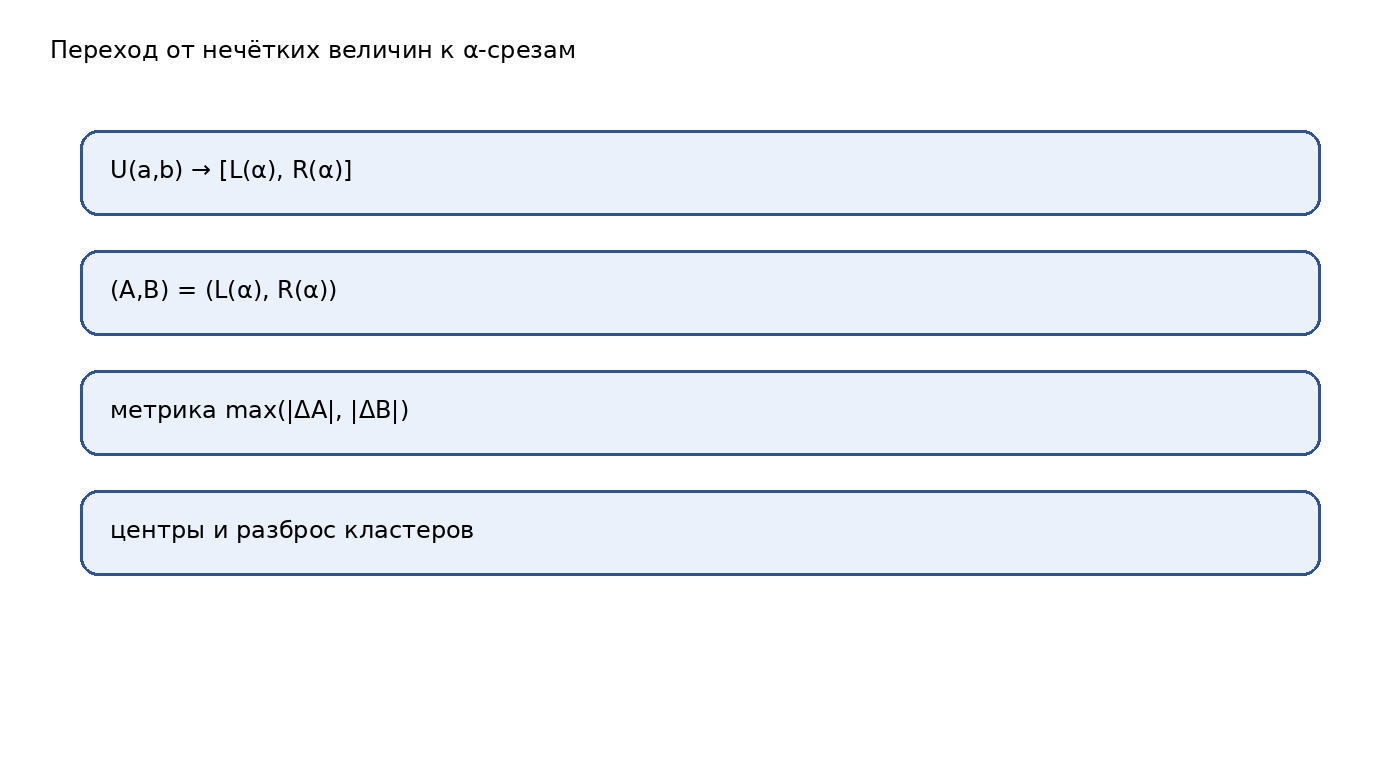
\includegraphics[width=0.9\textwidth]{figures/fig2_alpha.png}\caption{распределение α-срезов на плоскости (A,B)}\label{fig:2}\end{figure}

\subsection{Интервальная арифметика по принципу обобщения Заде}

Для непрерывной монотонной операции принцип обобщения Заде реализуется вычислением образа α-срезов. Пусть X\_α=[x\_1,x\_2], Y\_α=[y\_1,y\_2]. Тогда

\begin{equation}
(X+Y)_\alpha=[x_1+y_1,x_2+y_2],
\end{equation}

\begin{equation}
(X-Y)_\alpha=[x_1-y_2,x_2-y_1].
\end{equation}

Для произведения вычисляются четыре комбинации границ:

\begin{equation}
(XY)_\alpha=[\min P,\max P], \quad P=\{x_1y_1,x_1y_2,x_2y_1,x_2y_2\}.
\end{equation}

Для деления при $0\notin\operatorname{supp}Y$ используется умножение на обратный интервал:

\begin{equation}
(X/Y)_\alpha=X_\alpha\cdot[1/y_2,1/y_1].
\end{equation}

В \texttt{combine} сетка результата выбирается как максимум числа уровней двух операндов. На каждом уровне исходные срезы извлекаются через \texttt{cut\_at}, затем выполняется соответствующая операция. После этого для каждого i>0 левая граница заменяется на max(L\_i,L\_\{i−1\}), а правая — на min(R\_i,R\_\{i−1\}). Шаг восстанавливает вложенность при накоплении численной погрешности.

Деление с носителем делителя, содержащим ноль, блокируется в \texttt{fz\_apply}. Ошибка сохраняется в thread-local строке \texttt{g\_error}, а вызывающая сторона получает \texttt{NULL}. Это предотвращает формирование неограниченного или разрывного результата в модели, рассчитанной на конечные вложенные интервалы.

\subsection{Сравнение нечётких величин}

Сравнение возвращает знак разности центров тяжести:

\begin{equation}
\operatorname{cmp}(X,Y)=\operatorname{sign}(c_X-c_Y),
\end{equation}

при этом используется масштабируемый допуск

\begin{equation}
\varepsilon=10^{-9}\max(1,|c_X|,|c_Y|).
\end{equation}

Одновременно вычисляется степень возможности

\begin{equation}
\operatorname{Poss}(X\geq Y)= \sup_{u\geq v}\min(\mu_X(u),\mu_Y(v)).
\end{equation}

В дискретной реализации на общей сетке уровней проверяется условие R\_X(α)≥L\_Y(α), и максимальный подходящий α записывается в \texttt{degree}. В Go-слое операция сравнения выполняется в обоих направлениях, поэтому клиент получает \texttt{Poss(X≥Y)} и \texttt{Poss(Y≥X)}.

\subsection{Генерация случайных наборов}

В \texttt{rng.cpp} состояние xoshiro256** состоит из четырёх 64-битных слов. Инициализация выполняется четырьмя последовательными вызовами splitmix64 от исходного seed. Следующее состояние использует XOR-сдвиги и циклическую перестановку \texttt{rotl}, а выходное значение вычисляется как \texttt{rotl(s[1]*5,7)*9}.

Преобразование в число из [0,1) имеет вид

\begin{equation}
u=(x\mathbin{\gg}11)2^{-53}.
\end{equation}

Для генерации элемента выбираются

\begin{equation}
a\sim U[lo,hi],\qquad w\sim U[w_{min},w_{max}],\qquad b=a+w.
\end{equation}

\texttt{fz\_set\_generate} резервирует память под n элементов, создаёт величины через \texttt{make\_uniform} и записывает параметры генерации в журнал. Проверяются ограничения n∈[1,100000], lo≤hi и 0<w\_min≤w\_max.

\subsection{Отбор и кластеризация}

Отбор по ширине оставляет индексы, для которых

\begin{equation}
w_{min}\leq B_i-A_i\leq w_{max}.
\end{equation}

Отбор по окну оставляет интервалы, удовлетворяющие

\begin{equation}
x_1\leq A_i,\qquad B_i\leq x_2.
\end{equation}

В \texttt{selection.cpp} обе операции выполняют один линейный проход и записывают исходные индексы в пользовательский массив.

Алгоритм k-means++ принимает k и seed. Первый центр выбирается случайно. Для каждого следующего центра строится распределение вероятностей, пропорциональное квадрату расстояния до ближайшего выбранного центра. Затем выполняются назначение к ближайшему центру и пересчёт средних границ. Пустой кластер заполняется наиболее удалённым объектом. Цикл ограничен параметром \texttt{max\_iter}, а Go-обёртка передаёт 300 итераций.

Пороговый алгоритм не требует заранее заданного k. Сначала интервалы сортируются по A, затем последовательно относятся к ближайшему центру, если расстояние не превышает δ. Иначе создаётся новый кластер. Далее выполняется до 50 уточняющих проходов с переназначением объектов и пересчётом центров. После стабилизации метки перенумеровываются в порядке возрастания A.

---
\clearpage
\section{Глава 3. Архитектура и программная реализация}\subsection{Общая архитектура комплекса}

Система построена послойно. Внутренний слой содержит C++-структуры и алгоритмы. Граница между C++ и внешними языками проходит через \texttt{extern "C"} в \texttt{fuzzy.h}. Go-сервер вызывает этот интерфейс через cgo и отвечает за HTTP, JSON, импорт, экспорт и состояние пользовательского сеанса. HTML и JavaScript поставляются из \texttt{server/web} как встроенная файловая система. Десктопная программа запускает серверный бинарник на свободном loopback-порту и открывает адрес в CEF.

\begin{figure}[htbp]\centering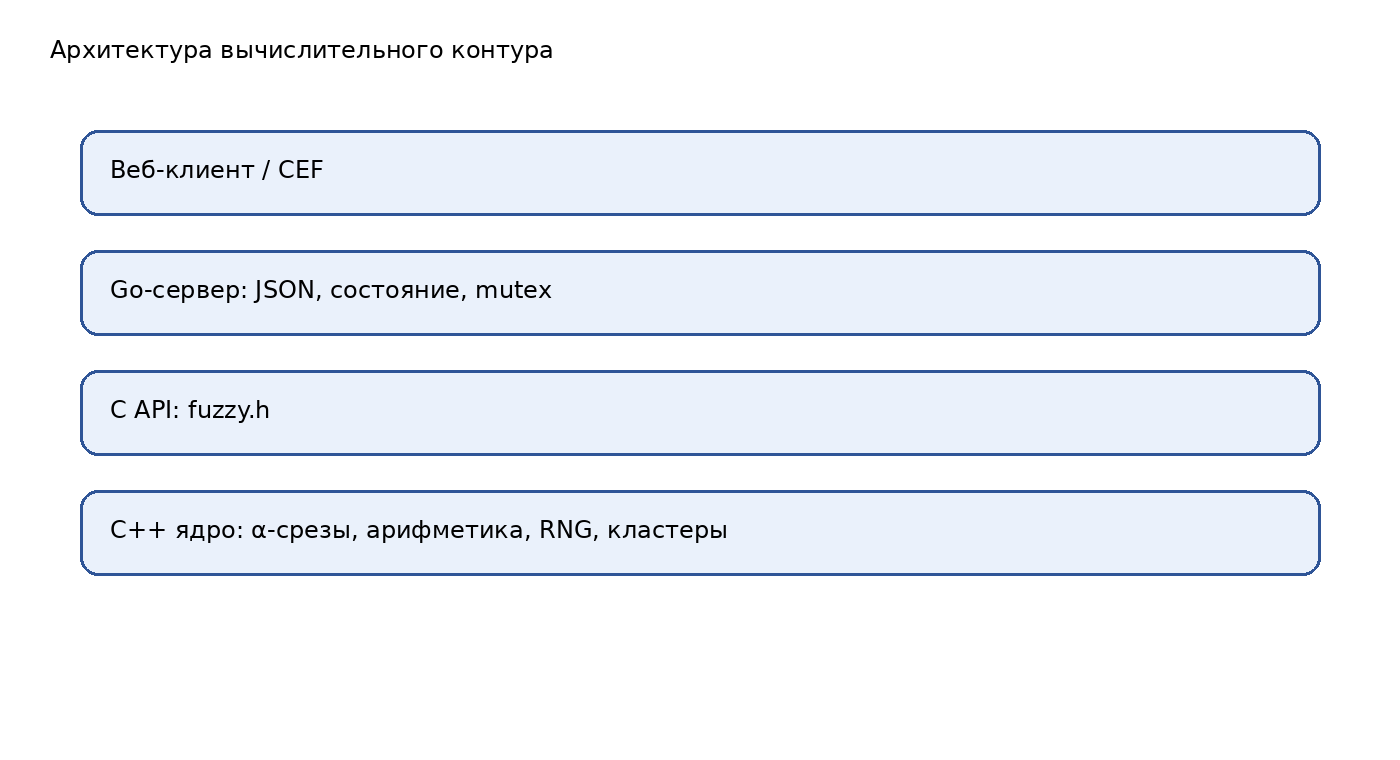
\includegraphics[width=0.9\textwidth]{figures/fig3_arch.png}\caption{схема архитектуры модуля кластеризации}\label{fig:3}\end{figure}

Сборка ядра описана в \texttt{fuzzy/CMakeLists.txt}. Создаются статическая \texttt{libfuzzy.a} и разделяемая \texttt{libfuzzy.so} из шести исходных файлов. Устанавливается C++17, включается position-independent code, применяются предупреждения \texttt{-Wall -Wextra}. Тестовый исполняемый файл связывается со статической библиотекой и регистрируется в CTest.

\subsection{Структуры данных C++}

\texttt{fz\_number} содержит флаг \texttt{uniform}, параметры \texttt{a} и \texttt{b}, а также векторы \texttt{left} и \texttt{right}. Для исходных U(a,b) параметры служат компактным каноническим представлением, а массивы хранят предвычисленные срезы. Для результатов операций \texttt{uniform=false}, параметры a и b не используются, а векторы описывают полную величину.

\texttt{fz\_set} содержит число уровней и \texttt{std::vector<fz\_number> items}. Вектор владеет объектами, поэтому освобождение набора освобождает все элементы без отдельного цикла в клиентском коде. Функция \texttt{fz\_set\_item} возвращает указатель, принадлежащий набору, и API явно запрещает освобождать его отдельно.

\texttt{fz\_rng} содержит четыре 64-битных слова состояния. Использование фиксированного размера исключает динамические аллокации в самом шаге генератора.

\subsection{Управление памятью и ошибки}

Объекты, созданные \texttt{fz\_create}, \texttt{fz\_create\_from\_cuts}, \texttt{fz\_clone}, операциями и генератором наборов, освобождаются парными функциями \texttt{fz\_free} и \texttt{fz\_set\_free}. Внутри ядра используются RAII-контейнеры \texttt{std::vector}, а C API предоставляет непрозрачные указатели. Такой контракт отделяет управление памятью C++ от Go-объектов.

Все функции, которые могут вернуть ошибку, очищают thread-local сообщение через \texttt{clear\_error}, затем записывают причину в \texttt{set\_error}. Go-функция \texttt{lastError} преобразует \texttt{fz\_last\_error()} в объект \texttt{error}. В HTTP-слое ошибки переводятся в JSON с кодом 400. В частности, отклоняются неверные диапазоны генерации, запросы с \texttt{a>=b}, неизвестные критерии, неверные методы и деление через ноль в носителе.

Журналирование синхронизировано мьютексом \texttt{g\_log\_mutex}. Каждая запись содержит локальное время, текст операции и немедленно сбрасывается в файл. Журналируются создание величин, арифметика, сравнения, генерация, отбор, кластеризация и ошибки.

\subsection{Реализация Go-оболочки и HTTP API}

В \texttt{server/fuzzy.go} через cgo подключается \texttt{fuzzy.h}, а параметры линейных массивов передаются в C как указатели на непрерывные участки Go-срезов. Функция \texttt{Generate} получает набор из C++ и копирует его в \texttt{[]Uniform}. \texttt{Intervals} создаёт временный C-набор, вычисляет срезы и копирует границы в два Go-среза. После возврата из функции C-объект освобождается через \texttt{defer}.

Сервер хранит \texttt{items}, \texttt{alpha}, массивы \texttt{left} и \texttt{right}, флаги отбора, метки кластеров, метод, число итераций и статистику кластеров. Все обработчики, изменяющие состояние, проходят через \texttt{handle}, который захватывает \texttt{sync.Mutex}, вызывает бизнес-операцию и формирует снимок \texttt{Snapshot}.

Основные маршруты имеют следующий смысл:

\begin{itemize}
\item \texttt{/api/generate} создаёт новый набор по seed и диапазонам;
\end{itemize}

\begin{itemize}
\item \texttt{/api/add}, \texttt{/api/clear}, \texttt{/api/import} изменяют набор;
\end{itemize}

\begin{itemize}
\item \texttt{/api/alpha} пересчитывает α-срезы без повторной генерации;
\end{itemize}

\begin{itemize}
\item \texttt{/api/select} применяет критерий ширины, окна или снимает отбор;
\end{itemize}

\begin{itemize}
\item \texttt{/api/cluster} запускает k-means++ либо пороговый алгоритм над выбранными интервалами;
\end{itemize}

\begin{itemize}
\item \texttt{/api/op} выполняет арифметику и сравнение двух U(a,b);
\end{itemize}

\begin{itemize}
\item \texttt{/api/export} выдаёт CSV с параметрами, срезами и метками;
\end{itemize}

\begin{itemize}
\item \texttt{/api/log} возвращает хвост журнала размером не более 256 KiB.
\end{itemize}

При любом изменении набора или α вызывается \texttt{recompute}. Он получает текущие интервалы из C API, выставляет все элементы выбранными и сбрасывает старые кластеры. Тем самым предотвращается использование меток, рассчитанных на другой α или другой состав данных.

\subsection{Веб-интерфейс и десктопный запускатель}

JavaScript-клиент строит графики на Canvas. Функции рисуют функции принадлежности, α-срезы, упорядоченные интервалы, плоскость (A,B), центры кластеров и результат арифметических операций. Данные поступают через JSON API и обновляют таблицы без перезагрузки страницы.

Десктопная часть использует CEF. \texttt{ServerProcess::Start} выбирает свободный loopback-порт, запускает \texttt{fuzzy-server} через \texttt{fork} и \texttt{execl}, ожидает доступность TCP-порта не более десяти секунд. Для корректного завершения дочернего процесса устанавливается \texttt{PR\_SET\_PDEATHSIG}, а при закрытии окна вызывается \texttt{Stop}, который сначала посылает SIGTERM и при необходимости SIGKILL. \texttt{FuzzyClient} обрабатывает заголовок окна, ошибки загрузки и загрузку CSV в каталог Downloads.

Такое разделение сохраняет единый вычислительный и серверный контур для браузерного и десктопного режимов. Различается только способ отображения страницы и жизненный цикл локального сервера.

\begin{figure}[htbp]\centering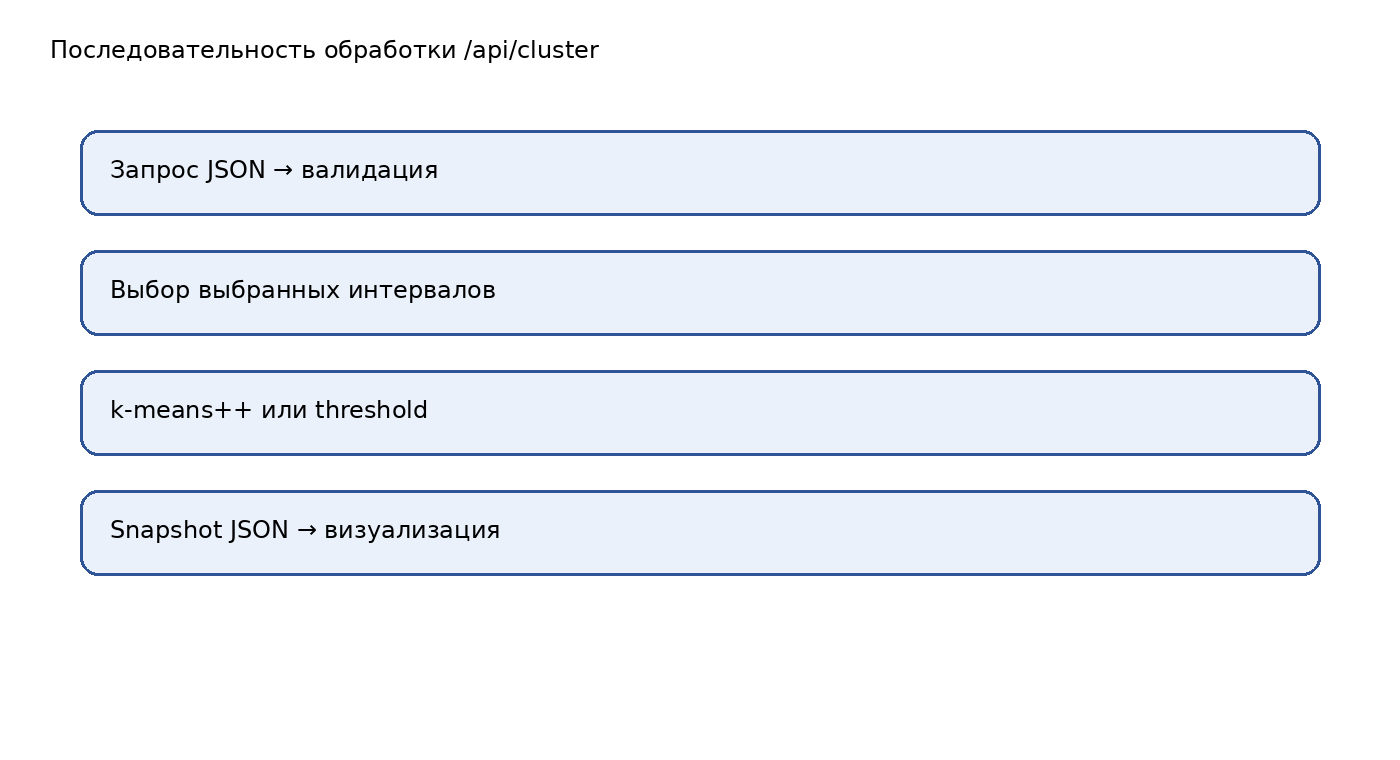
\includegraphics[width=0.9\textwidth]{figures/fig4_sequence.png}\caption{последовательность обработки запроса /api/cluster}\label{fig:4}\end{figure}

\subsection{Оценка вычислительной сложности}

Пусть n — число интервалов, k — число кластеров, m — число α-уровней.

\begin{itemize}
\item построение U(a,b) и вычисление одного α-среза имеют сложность O(m) и O(1) соответственно;
\end{itemize}

\begin{itemize}
\item получение всех α-срезов набора имеет сложность O(n);
\end{itemize}

\begin{itemize}
\item отбор по ширине и окну имеет сложность O(n);
\end{itemize}

\begin{itemize}
\item одна итерация k-means имеет сложность O(nk), а инициализация k-means++ — O(nk);
\end{itemize}

\begin{itemize}
\item пороговая кластеризация требует сортировки O(n log n) и до 50 проходов, каждый из которых в общем случае имеет сложность O(nk);
\end{itemize}

\begin{itemize}
\item расчёт статистики кластеров выполняется за O(n+k).
\end{itemize}

Память k-means составляет O(n+k), порогового алгоритма — O(n+k). Временная стоимость передачи через cgo определяется копированием результатов и не меняет асимптотику алгоритмов. Фиксированный размер 21 уровня в Go-сервере ограничивает объём JSON, тогда как C API поддерживает более плотную сетку.

---
\clearpage
\section{Глава 4. Экспериментальное исследование и результаты}\subsection{Методика тестирования}

Верификация выполнена на исходном тестовом наборе \texttt{fuzzy/tests/test\_main.cpp}. Сборка проведена командой \texttt{make test}, которая конфигурирует CMake в режиме Release, собирает статическую и разделяемую библиотеки, компилирует \texttt{fuzzy\_tests} и запускает CTest.

Тесты охватывают следующие свойства:

\begin{enumerate}
\item Для U(0,10) проверяются α-срез [7,10] при α=0.7, значения функции принадлежности внутри и вне носителя, а также центр тяжести 20/3.
\item Для арифметики проверяются границы суммы, разности, произведения и частного, интерполированное значение принадлежности и ошибка деления через величину с носителем [-1,1].
\item Для сравнения проверяются знаки центров тяжести и степени возможности для пересекающихся и удалённых величин.
\item Для генератора проверяется диапазон [0,1), среднее 100000 значений, совпадение последовательностей при одинаковом seed и диапазоны параметров 300 сгенерированных величин.
\item Для отбора проверяется выполнение ограничений ширины и окна для каждого возвращённого индекса.
\item Для кластеризации создаются три группы по 30 интервалов вокруг центров 0, 50 и 100. Проверяется согласованность меток внутри групп, различие меток между группами, автоматическое получение трёх кластеров при δ=10 и одного кластера при δ=1000.
\end{enumerate}

Все тестовые условия проходят без ошибок: исполняемый файл сообщил \texttt{100982/100982 checks passed}, а CTest завершил единственный зарегистрированный тест со статусом \texttt{Passed}. Изменение seed изменяет псевдослучайную последовательность, но не нарушает диапазоны и инварианты алгоритмов.

\subsection{Контрольный замер вычислительной эффективности}

Для оценки порядка времени исполнения дополнительно собрана небольшая программа с \texttt{-O2}, связывающаяся с \texttt{build/libfuzzy.a}. На каждой итерации генерировался набор с seed=42, параметрами lo=0, hi=100, w\_min=5, w\_max=30 и 21 уровнем. Затем измерялись генерация и получение α-срезов при α=0.7, k-means++ для k=3 и пороговый алгоритм при δ=5.

\begin{table}[htbp]
\centering
\caption{Контрольные измерения вычислительной эффективности}
\label{tab:perf}
\begin{tabular}{rrrrr}
\toprule
$n$ & Генерация и срезы, мс & $k$-means++, мс & Итерации & Число кластеров \\
\midrule
50 & 0,014 & 0,005 & 10 & 18 \\
100 & 0,011 & 0,003 & 4 & 18 \\
300 & 0,038 & 0,005 & 3 & 22 \\
1000 & 0,119 & 0,071 & 19 & 22 \\
5000 & 1,098 & 0,520 & 28 & 26 \\
\bottomrule
\end{tabular}
\end{table}

Измерения характеризуют один запуск на локальной машине и предназначены для проверки порядка величин, а не для публикации аппаратно независимого бенчмарка. Небольшой разброс между n=50 и n=100 объясняется дискретностью таймера и стоимостью запуска. Начиная с n=300 наблюдается ожидаемое увеличение времени. Пороговая кластеризация в выбранной конфигурации дороже k-means++ из-за сортировки, последовательных уточняющих проходов и динамического числа кластеров.

При n=5000 k-means++ завершился за 0,520 мс после 28 итераций. Пороговый метод занял 11,793 мс и сформировал 26 кластеров при δ=5. Результаты соответствуют различию алгоритмических контуров и не свидетельствуют о деградации памяти в проверенном диапазоне.

\begin{figure}[htbp]\centering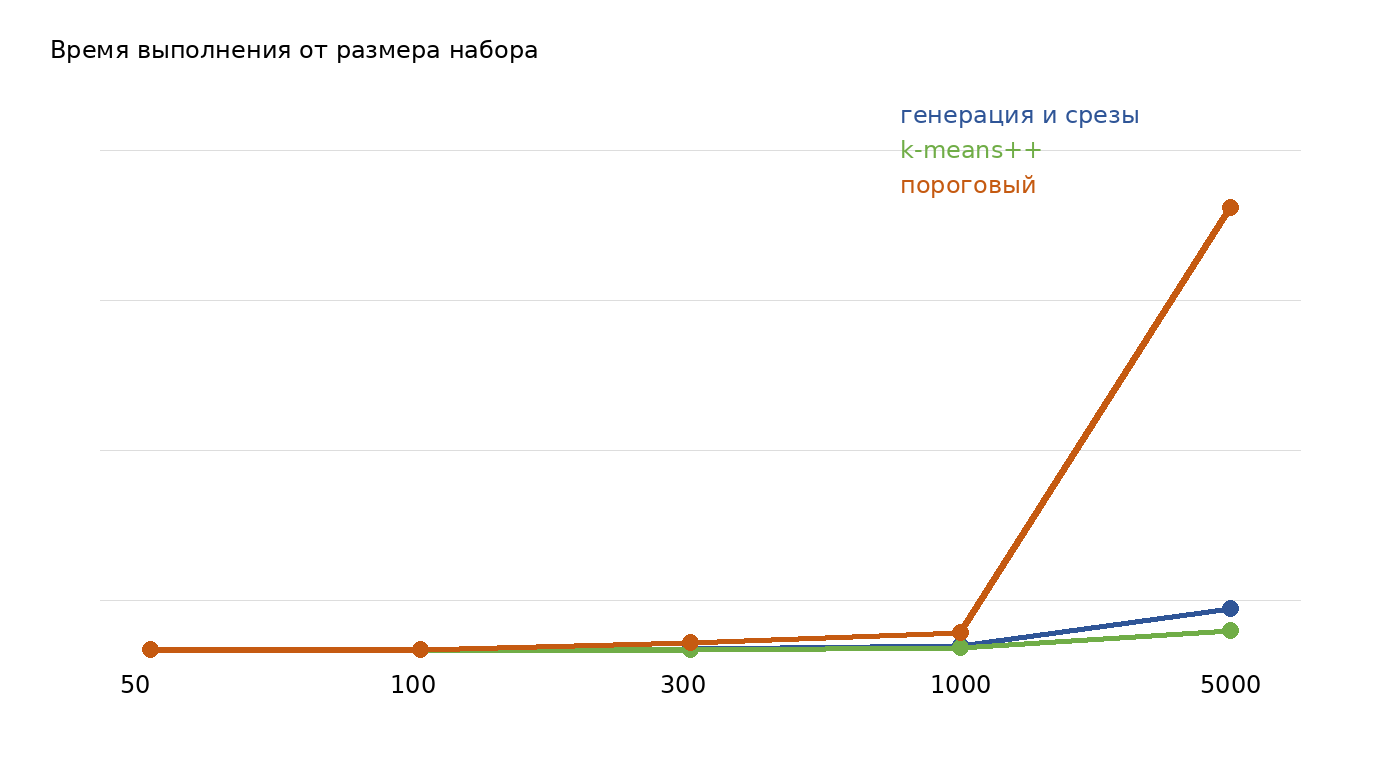
\includegraphics[width=0.9\textwidth]{figures/fig5_time.png}\caption{время выполнения от размера набора}\label{fig:5}\end{figure}

\subsection{Интерпретация результатов кластеризации}

В тесте с тремя синтетическими группами интервалы построены около центров 0, 50 и 100 с малым случайным шумом. k-means++ при k=3 присваивает соседние элементы одной группе одинаковые метки, а три группы получают разные метки. Это показывает, что метрика max(|ΔA|,|ΔB|) согласованно различает разнесённые облака интервалов.

Пороговый алгоритм при δ=10 также выделяет три кластера. Увеличение δ до 1000 приводит к объединению всех объектов в один кластер, поскольку расстояние до единого центра оказывается ниже порога. Тем самым параметр δ управляет компромиссом между компактностью и числом групп. В прикладном запуске δ следует выбирать в масштабе исходной переменной, поскольку он измеряется в тех же единицах, что и A и B.

Для случайного набора из 5000 интервалов при δ=5 число кластеров оказалось равным 26. Это число не является универсальной характеристикой генератора. Оно зависит от seed, диапазона a, диапазона ширин и выбранного α. При увеличении α длина среза уменьшается, что обычно уменьшает вертикальный разброс точек на плоскости (A,B), однако сдвиг A вправо может изменить относительное расположение групп.

\begin{figure}[htbp]\centering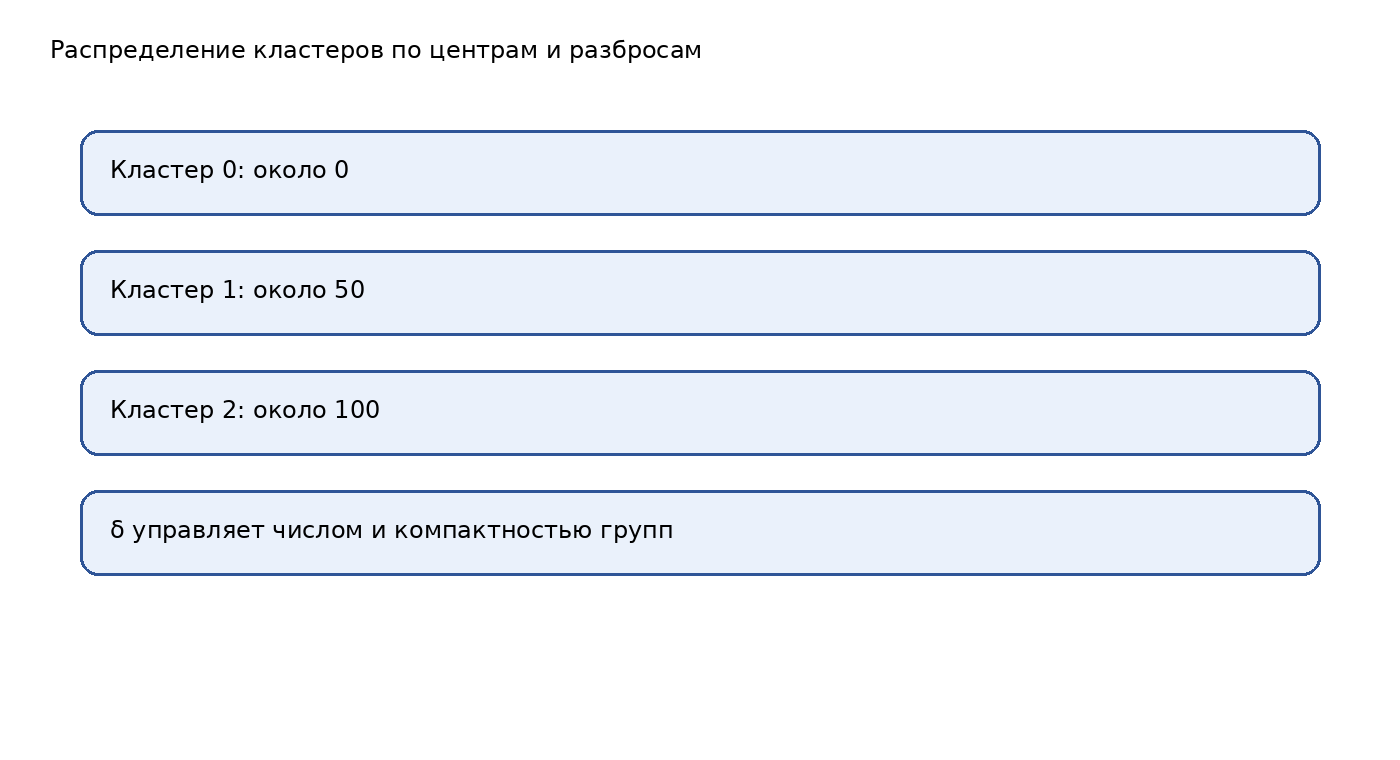
\includegraphics[width=0.9\textwidth]{figures/fig6_clusters.png}\caption{распределение кластеров по центрам и разбросам}\label{fig:6}\end{figure}

\subsection{Проверка корректности интерфейсного контура}

Сервер собирается командой \texttt{make server}, которая сначала собирает библиотеку, затем запускает \texttt{go build -a} с включённым cgo. При обращении к \texttt{/api/generate} параметры запроса проверяются на стороне Go и C++. Снимок состояния содержит исходные a,b, текущий α-срез, признак отбора и метку кластера. После изменения α прежние метки сбрасываются, что исключает рассогласование между данными и визуализацией.

Операционный маршрут \texttt{/api/op} создаёт две величины U(a,b), возвращает исходные срезы, результат операции, центр тяжести, сравнение и два значения Poss. При запрещённом делении результат содержит текст ошибки, полученный из \texttt{fz\_last\_error}, а HTTP-обработчик сохраняет корректный JSON-контракт.

Импорт CSV принимает разделители запятую, точку с запятой, табуляцию и пробел. Экспорт включает столбцы \texttt{id,a,b,A,B,selected,cluster}. Это позволяет использовать результат кластеризации в последующем внешнем анализе.

\subsection{Ограничения экспериментальной части}

Проведённые измерения не заменяют профилирование на целевом оборудовании. В проекте отсутствуют стресс-тесты на многопоточные запросы к серверу, поэтому синхронизация подтверждена анализом кода и сборкой, но не нагрузочным экспериментом. Не исследовалась чувствительность качества кластеров к систематическому изменению α, k и δ по сетке параметров. Эти направления относятся к расширенному исследованию и могут быть включены в выпускную квалификационную работу.

---\clearpage
\section*{Заключение}\addcontentsline{toc}{section}{Заключение}В курсовом проекте реализован согласованный вычислительный контур для работы с нечёткими величинами на основе U(a,b). C++-ядро задаёт математическую модель, реализует хранение α-срезов, интервальную арифметику, сравнение, генерацию и кластеризацию. C API делает ядро доступным из Go, а Go-сервер обеспечивает проверку запросов, синхронное состояние и HTTP-интеграцию. Веб-интерфейс и CEF-оболочка используют один и тот же серверный контракт.

Поставленные задачи выполнены. Проверки \texttt{fuzzy\_tests} подтверждают корректность базовых инвариантов: вложенность срезов, границы операций, воспроизводимость генератора, корректность отбора и устойчивое разделение синтетических кластеров. Контрольные измерения показывают миллисекундное время обработки наборов до 5000 интервалов в Release-сборке, при этом пороговая кластеризация закономерно требует больше времени, чем k-means++ с фиксированным k.

Практическая область применения модуля включает учебные эксперименты, анализ интервалов с неопределёнными границами и прототипирование алгоритмов нечёткого кластерного анализа. При переходе к промышленной нагрузке потребуются расширенные бенчмарки, анализ устойчивости к выбору α и δ, а также отдельное хранилище состояния.

---\clearpage
\nocite{batyrshin2007,demidova,abchuk1979,zadeh1965,arthur2007,blackman2021}\printbibliography[title={Список использованных источников}]\addcontentsline{toc}{section}{Список использованных источников}
\end{document}
